% I have provided the source and required media for this presentation
% under the hope that it will be useful. Please don't use it for
% anything nefarious.

% Also, note that this LaTeX file requires the beamer class to
% compile. If you don't already have it, you are expected to obtain
% and install it from http://latex-beamer.sourceforge.net/

% (c) 2011 -- Harish Narayanan

\documentclass[ignorenonframetext]{beamer}

\usepackage{graphicx}
\usepackage{amsfonts}
\usepackage{amssymb}
\usepackage{fancyvrb}
\usepackage{color}
\usepackage{multimedia}
\usepackage[english]{babel}
\usepackage[latin1]{inputenc}
\usepackage{textcomp}

% Custom commands

\newcommand{\references}[1] {
  \begin{flushright}
    \scriptsize [#1] \normalsize
  \end{flushright}
}

\newcommand{\addfigure} {
  \scriptsize
  \textcolor{red}{[insert figure]}
  \normalsize
}

\newcommand{\fixme} {
  \scriptsize
  \textcolor{red}{[fix me]}
  \normalsize
}

% All sorts of things pertinent to styling beamer
\usetheme{boxes}
\setbeamertemplate{navigation symbols}{}
\usecolortheme{seagull}
\usefonttheme{professionalfonts}
\useinnertheme{circles}
\setbeamercolor{frametitle}{fg=red}
\setbeamercolor{title}{fg=red}

\mode<presentation> {
  \setbeamercovered{transparent}
}

\title{Electrophysiological modelling of chondrocytes in human
  articular cartilage}
\author{H.~Narayanan}
\subject{}
\institute[]{}
\date[]{}

\begin{document}

% 0. Title slide and mapping
%
%   Electrophysiological modelling of chondrocytes in human articular
%   cartilage
%
%   - Introducing the chondrocyte and why it is interesting in the
%     context of cartilage
%   - Some particular scientific questions
%
%   - Model and motivation
%   - Preliminary results
%   - Discussion

%\frame{\titlepage}

% Mapping slide containing visual outline
\begin{frame}
  \frametitle{This talk will describe the status of our
    electrophysiological model of chondrocytes in human articular
    cartilage}
  \begin{columns}
    \begin{column}{3cm}
      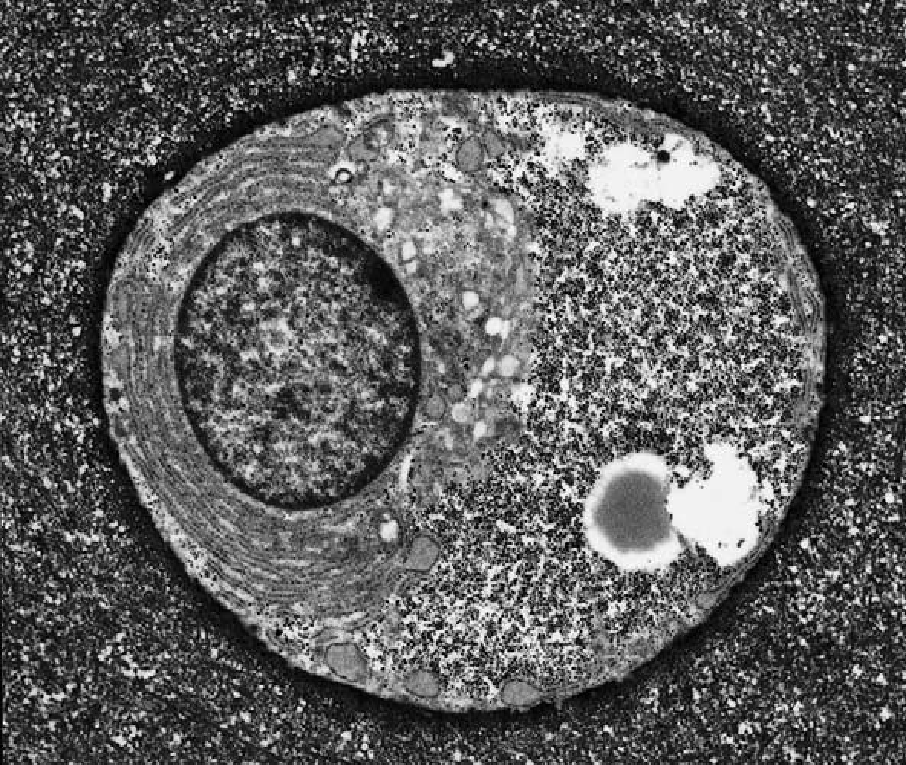
\includegraphics[width=3cm]{../images/pdf/chondrocyte-micrograph}
    \end{column}
    \begin{column}{9cm}
      What is the chondrocyte, and why is it interesting?
    \end{column}
  \end{columns}
  \vspace{0.3cm}
  \begin{columns}
    \begin{column}{1cm}
      % Empty
    \end{column}
    \begin{column}{2.5cm}
      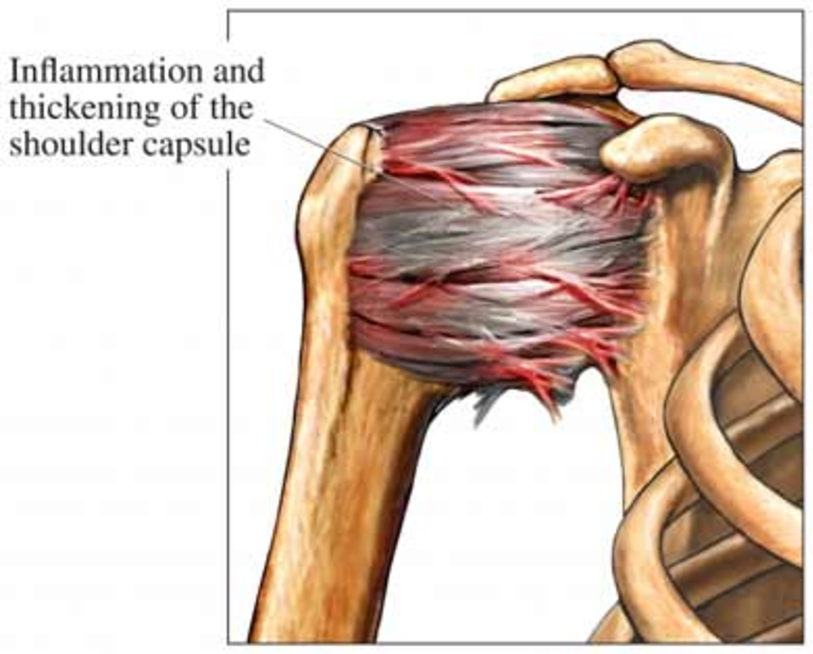
\includegraphics[width=2.5cm]{../images/pdf/frozen-shoulder}
    \end{column}
    \begin{column}{0.1cm}
      % Empty
    \end{column}
    \begin{column}{8.5cm}
      What are the specific questions we aim to answer?
    \end{column}
  \end{columns}
  \vspace{0.3cm}
  \begin{columns}
    \begin{column}{2cm}
      % Empty
    \end{column}
    \begin{column}{2cm}
      \includegraphics[width=2.5cm]{../results/pdf/membrane_behaviour}
    \end{column}
    \begin{column}{0.5cm}
      % Empty
    \end{column}
    \begin{column}{8cm}
      How does our model help us answer these questions?
    \end{column}
  \end{columns}
\end{frame}

% 1. What is the chondrocyte and why is it interesting?

\begin{frame}{Articular cartilage is the connective tissue that
    separates bones at joints, allowing them to slide past each other}

  \begin{columns}

    \begin{column}{6cm}
      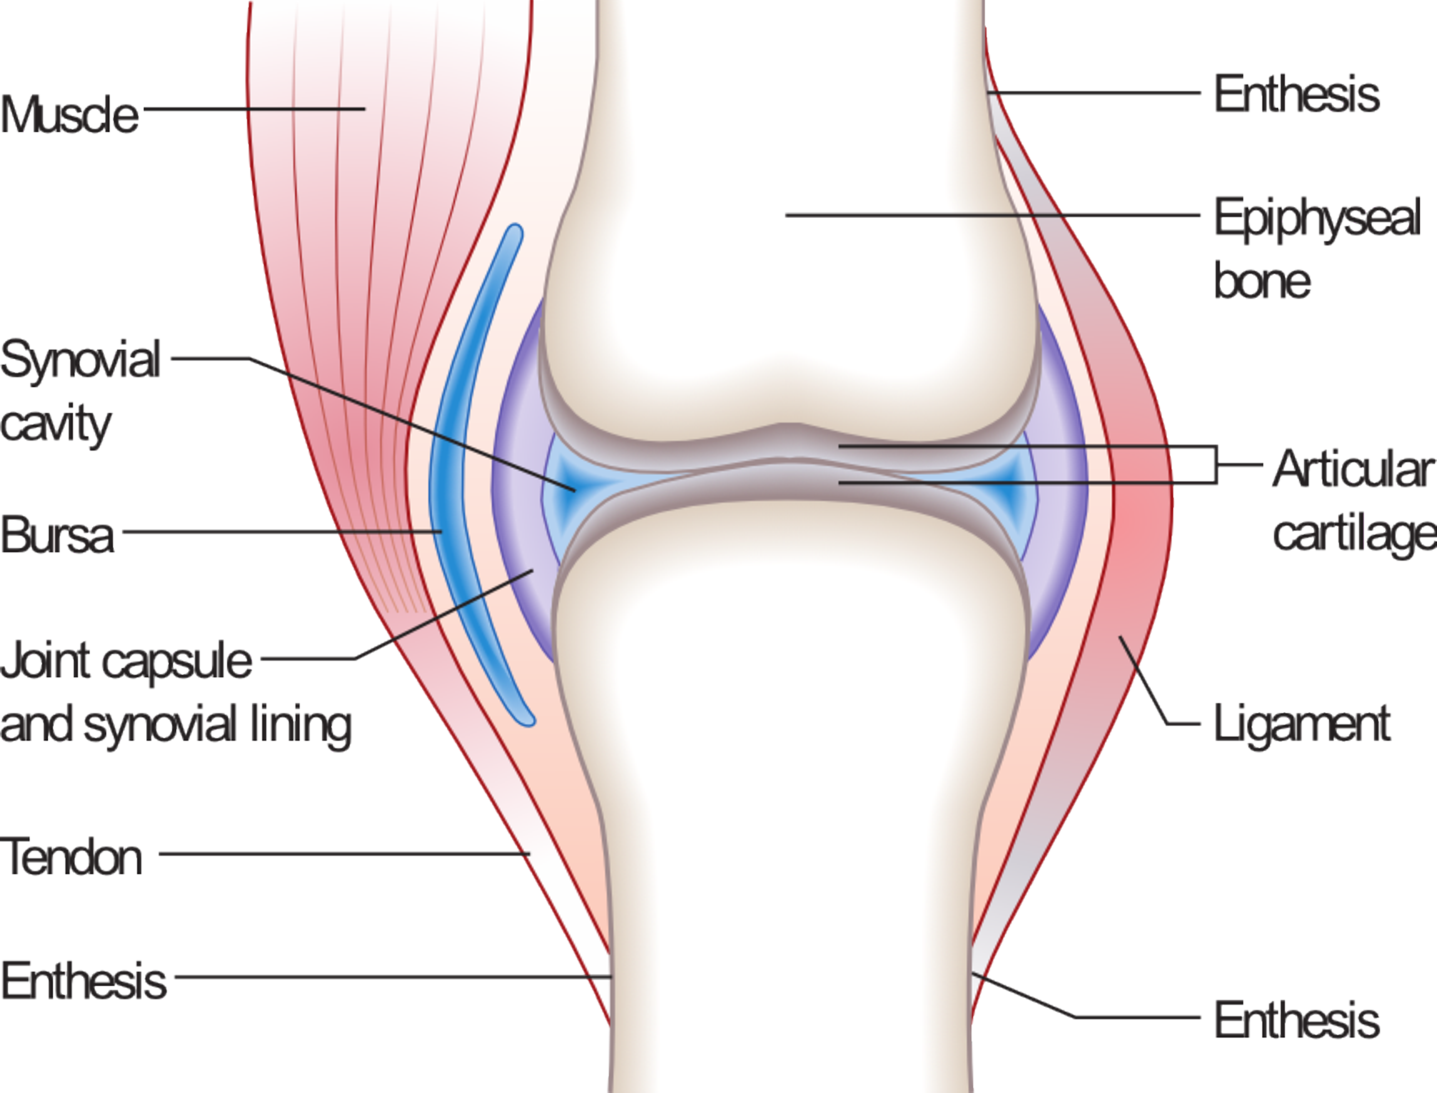
\includegraphics[width=6cm]{../images/pdf/joint}
    \end{column}

    \begin{column}{6cm}
      \begin{itemize}
      \item <1-> Cartilage is composed of {\em chondrocytes}, an ECM
        (collagen and elastin) and proteoglycans\\[0.5cm]
        \pause
      \item<2-> The tissue is aneural, avascular and alymphatic and is
        thus slow to grow and heal
        % and relatively easy to study mathematically?
      \end{itemize}
    \end{column}

  \end{columns}

  \references{Poole, 1997}

\end{frame}

\begin{frame}{Chondrocytes are the resident cells of articular
    cartilage and are responsible for maintaining the extracellular
    matrix}

 \begin{columns}

    \begin{column}{6cm}
      \begin{center}
      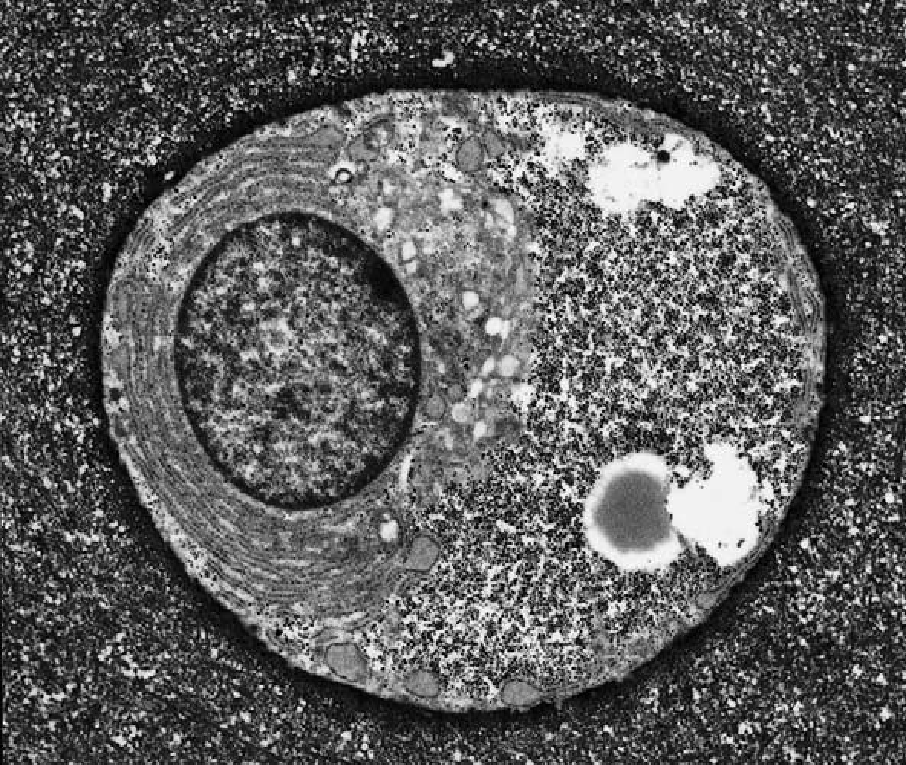
\includegraphics[width=6cm]{../images/pdf/chondrocyte-micrograph}
      {\\[-0.1cm] \scriptsize Electron micrograph of typical chondrocyte}
      \end{center}
    \end{column}

    \begin{column}{6cm}
      \begin{itemize}
      \item<1-> Chondrocytes are isolated within a voluminous
        ECM
      \item<1-> Relies on diffusion from the articular surface for
        nutrient and metabolite exchange\\[0.5cm]
        \pause
      \item<2-> Sensitive to extra-cellular pH, ionic environment,
        stress state
      \item<2-> Arthritis is the associated degenerative pathology
      \end{itemize}
    \end{column}

  \end{columns}

  \references{Archer \& Francis-West 2003}

\end{frame}

% A lot can happen, but we are interested in something particular
%
% 2. The specific question(s) we want to answer

\begin{frame}{We narrow our focus to a few specific questions to
    motivate our initial modelling efforts}

  \begin{columns}
    \begin{column}{6cm}
      \begin{center}
        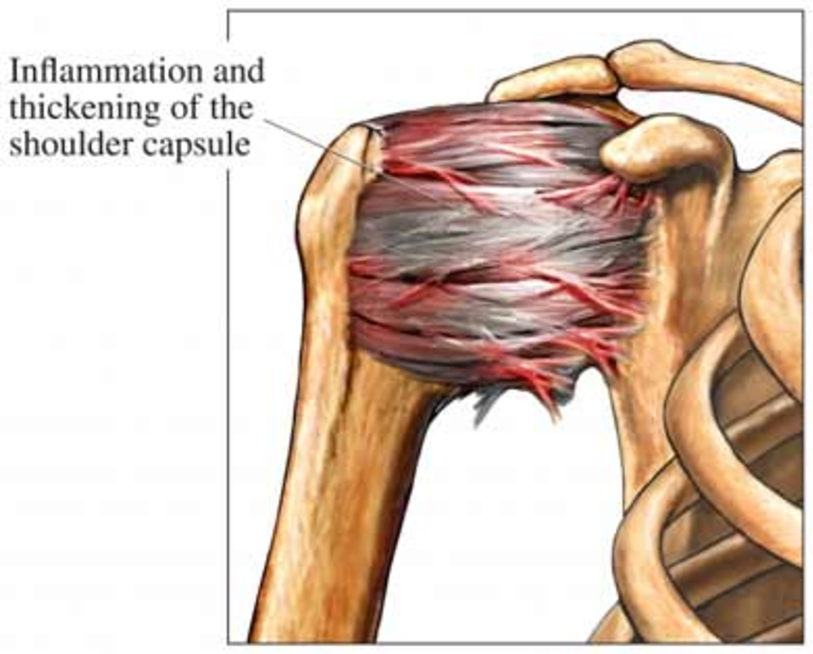
\includegraphics[width=4cm]{../images/pdf/frozen-shoulder}
      \end{center}
    \end{column}
    \begin{column}{6cm}
      What causes the ``frozen shoulder syndrome''
      when tissue is exposed to the local an\ae{}sthetic
      bupivacaine?
    \end{column}
  \end{columns}

  \vspace{0.5cm}

  \begin{itemize}
    \pause
  \item<2-> Hypothesis 2: pH and volume regulation (via ASIC) \fixme
  \item<2-> Hypothesis 3: Apoptosis and osteoarthritis?
    \fixme
  \end{itemize}
  \references{Webb, 2009; Lewis et al., 2011; citation 3}

\end{frame}

\begin{frame}{In order to answer such questions, we need a model that
    helps us understand some fundamental things}
  \begin{itemize}
  \item The important important ion channels for the cell\\[0.5cm]
  \item The basis of the resting membrane potential\\[0.5cm]
  \item How this potential relates to cellular volume regulation\\[0.5cm]
  \end{itemize}
\end{frame}

% There is a dearth of good biophysical models for this cell type and
% so we construct our own.
%
% But this is not so easy because in physiology literature, the cell
% channelome is quite complex
%
% Return to review papers. As of 1996, it looked like [figure], and as
% of 2011 people feel it looks like [figure], so on the whiteboard in
% my office you have a superset of these studies.
%
% 3. Modelling the electrophysiology of a single cell

\begin{frame}{Physiology literature gives us a broad overview of the
    ion channels present in chondrocytes}

  \vspace{0.4cm}
  \includegraphics[width=\textwidth]{../images/pdf/chondrocyte-channelome}

  \references{Hall et al., 1996; Barrett-Jolley et al., 2010}

\end{frame}

%  Talk about some important ones and what their roles might be.

\begin{frame}{And so, we started on my whiteboard with a superset of
    all the channels experimentalists were talking about \ldots}

  \addfigure

\end{frame}

%
% And so, this is the model that is being researched and
% implemented. Removing the things that are not pertinent to humans
% etc., we end up with the following initial model.
%
% 4. The computational model

\begin{frame}{\ldots{} simplified things a little, and arrived at our
    electrophysiological model of a single chondrocyte}

  \begin{center}
    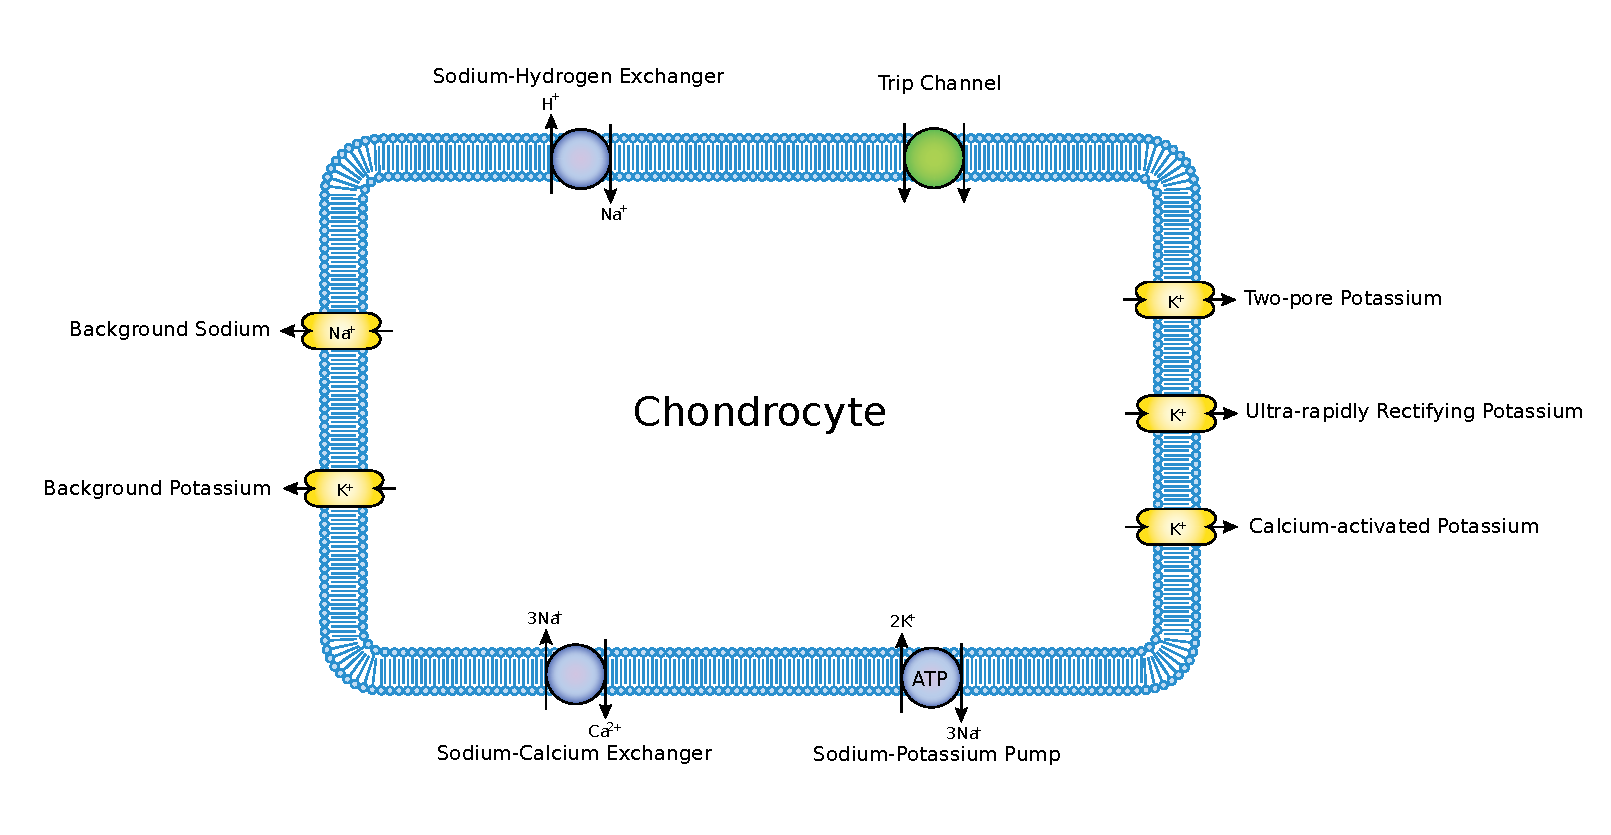
\includegraphics[width=\textwidth]{../images/pdf/chondrocyte-model-cellml}
    {\\[-0.1cm] \scriptsize Our ion channel model of a single chondrocyte \fixme}
  \end{center}

\end{frame}


\begin{frame}{\ldots{} simplified things a little, and arrived at our
    electrophysiological model of a single chondrocyte}

  \begin{equation*}
    \begin{split}
      -C_{\rm m} \frac{dV_{\rm m}}{dt} = & \phantom{+\,} \underbrace{I_{\rm Na_b} + I_{\rm K_b}}_{\rm Background\, currents}\\
      & +\, \underbrace{I_{\rm NaK} + I_{\rm NaCa} + I_{\rm NaK}}_{\rm Pumps\, and\, exchangers}\\
      & +\, \underbrace{I_{\rm K_{ur}} + I_{\rm K_{2\, pore}} + I_{\rm K_{Ca-act}} + I_{\rm K_{ATP}}}_{\rm Potassium\, channels}\\
      & +\, \underbrace{I_{\rm ASIC} + I_{\rm TRP1} + I_{\rm TRP2} + I_{\rm stim}}_{\rm Other\, currents}
    \end{split}
  \end{equation*}

  \vspace{0.5cm}
  \pause
  For more details on the model and how it is implemented, let us step
  into the code for a quick demo

\end{frame}


% 1. Discuss some functional forms, including rationale
% 2. ODE Solver
% 3. Code layout
% 4. Return to one specific hypothesis and point out the channels that
%    seem important -- \references{functional forms, Clark et. al,
%    parameter estimation}
% 4. Parameter estimation; genetic algorithm idea?

% And with these parameters, I observe the following behaviour in my
% test cases
%
% 5. Some numerical simulations and their implications

\begin{frame}{At the moment, I am completing the implementation and
    starting to tune parameters}

  \vspace{-0.4cm}

  \begin{center}
    \includegraphics[width=0.9\textwidth]{../results/pdf/membrane_behaviour}
  \end{center}

  \references{parameter estimation, benchmarking, hypothesis}

\end{frame}

% 6. Discussion

\begin{frame}{In conclusion, \ldots}

  \begin{itemize}
  \item Summarise what has been done
    \begin{itemize}
      \item Learnt a bit about the physiology of the chondrocyte
      \item Some ideas of the channels involved
      \item Arrived at some interesting questions
      \item A basic model to answer these questions
    \end{itemize}
  \item For the future
    \begin{itemize}
    \item Ask for modelling advice
    \item Implications of the calculations
    \item Tissue level models and stress response
    \end{itemize}
  \end{itemize}

  \references{{\tt https://bitbucket.org/harish/chondrocyte-model/}}

\end{frame}

\end{document}

% Local Variables:
% mode: latex
% mode: flyspell
% mode: auto-fill
% End: